\documentclass{article}
\usepackage{iclr2026_conference,times}
\input{math_commands.tex}
\usepackage{hyperref}
\usepackage{url}
\usepackage{booktabs}
\usepackage{graphicx}
\usepackage{microtype}

\raggedbottom

\title{Hierarchical Failure Containment for Long-Horizon Robot Policies}
\author{Anonymous Authors}

\begin{document}
\maketitle

\begin{abstract}
Long-horizon robot tasks fail badly when low-level execution errors corrupt higher-level task state: a slipping grasp invalidates an assembly subgoal, a contact instability damages a part, or an exhausted recovery budget turns a local mistake into a task-level cascade. Hierarchical policies and option termination help, but they do not by themselves decide where a failure should be contained. We rebuild Paper 105 around a falsifiable claim: hierarchical robot policies should explicitly model containment boundaries between low-level skill anomalies, mid-level subgoals, and high-level task state. The local benchmark covers 5 robot task families, 7 failure regimes, 5 stress splits, 9 methods, 7 seeds, and 84 episodes per group. On combined cascade stress, the proposed containment graph obtains $0.576 \pm 0.007$ success versus $0.492 \pm 0.006$ for the strongest non-oracle baseline, while improving containment from $0.394$ to $0.515$, reducing state corruption from $0.098$ to $0.053$, and reducing damage from $0.050$ to $0.029$. Pairwise tests favor the proposed method over the strongest baseline in 7/7 seeds, and ablations show that local containment edges, cross-level escalation, recovery-budget memory, corruption prediction, and false-halt calibration each matter. A 2026-06-15 continuation audit reran the full benchmark and preserved the terminal decision: \textbf{STRONG\_REVISE}. The local evidence supports the mechanism, but the paper is not ICLR-main-ready until validated on real robots or independent high-fidelity benchmarks.
\end{abstract}

\section{Motivation}
Hierarchical robot policies are attractive because long tasks naturally decompose into skills, options, or subgoals. The options framework formalized temporally extended actions \citep{sutton1999options}, and later work learned option policies and termination functions directly \citep{bacon2017option}. HIRO-style methods further showed that hierarchical policies can be data-efficient for difficult simulated robotic control tasks \citep{nachum2018hiro}. But hierarchy alone does not solve failure containment. A low-level retry may be safe in one skill and task-corrupting in another; a high-level halt may protect the task but waste valid execution.

Recovery work addresses adjacent problems. Recovery RL separates task and recovery policies for safety \citep{thananjeyan2020recovery}, RecoveryChaining learns local recovery policies for manipulation \citep{vats2024recoverychaining}, and recent VLA recovery systems generate executable recovery actions for failures \citep{lin2025failsafe}. Paper 105 asks a narrower question: can a hierarchy diagnose the level at which a failure should be contained before it cascades into high-level state corruption?

\section{Method sketch}
The proposed method is a hierarchical failure containment graph. Nodes represent low-level controller anomalies, skill-local precondition drift, mid-level subgoal validity, high-level task-state corruption, recovery budget, and false-halt risk. Edges represent cross-level cascade paths. The monitor scores:
\begin{itemize}
\item local containment feasibility,
\item cross-level escalation necessity,
\item remaining recovery budget,
\item task-state corruption risk,
\item false-halt cost, and
\item recovery utility.
\end{itemize}

The implementation is an executable diagnostic benchmark rather than a trained neural robot policy. That is enough for a local mechanism audit, but it is not enough for a main-conference empirical robotics claim.

\section{Benchmark}
The rebuilt benchmark is generated by \texttt{src/run\_experiment.py}. It writes aggregate CSVs and figures directly, so the full run remains lightweight without dropping tasks, regimes, baselines, seeds, ablations, or stress tests.

\paragraph{Tasks.}
The tasks are drawer retrieval, peg assembly, mobile manipulation delivery, tool-use sequence, and bimanual handoff.

\paragraph{Failure regimes.}
The regimes are actuator slip, perception glitch, contact instability, precondition drift, subgoal drift, recovery-budget exhaustion, and cross-level cascading failure.

\paragraph{Splits.}
The stress splits are nominal, low-level perturbation, mid-level subgoal shift, delayed escalation, and combined cascade stress.

\paragraph{Methods.}
The baselines are flat behavior cloning, hierarchy without containment, local safety filtering, reactive retry recovery, uncertainty halting, option-termination monitoring, and a failure-aware hierarchical controller. The benchmark also includes the proposed hierarchical containment graph and an oracle containment supervisor.

\paragraph{Metrics.}
The evidence reports task success, containment rate, state corruption, cascade rate, damage, false halt, recovery success, escalation precision, containment latency, recovery cost, regret to oracle, paired seed differences, ablations, stress sweeps, and failure cases.

\section{Results}
% Auto-generated by src/run_experiment.py
\begin{table}[t]
\centering
\caption{Combined-cascade hierarchical-failure-containment benchmark.}
\begin{tabular}{lrrrrrr}
\toprule
Method & Succ. & Contain & Corrupt & Cascade & Dmg. & Regret \\
\midrule
Oracle & 0.734 & 0.629 & 0.012 & 0.071 & 0.006 & 0.000 \\
Proposed & 0.576 & 0.515 & 0.053 & 0.116 & 0.029 & 0.159 \\
FailAwareHC & 0.492 & 0.394 & 0.098 & 0.158 & 0.050 & 0.242 \\
OptionTerm & 0.442 & 0.338 & 0.116 & 0.179 & 0.063 & 0.292 \\
UncertHalt & 0.389 & 0.290 & 0.143 & 0.197 & 0.071 & 0.346 \\
ReactiveRetry & 0.382 & 0.269 & 0.146 & 0.213 & 0.071 & 0.353 \\
SafetyFilter & 0.349 & 0.275 & 0.156 & 0.221 & 0.082 & 0.385 \\
NoContain & 0.306 & 0.177 & 0.179 & 0.255 & 0.096 & 0.429 \\
FlatBC & 0.232 & 0.113 & 0.207 & 0.264 & 0.106 & 0.503 \\
\bottomrule
\end{tabular}
\end{table}


The strongest non-oracle baseline is \texttt{failure\_aware\_hierarchical\_controller}. On combined cascade stress, the proposed method improves success by $0.084 \pm 0.009$, wins 7/7 paired seeds, improves containment by $0.121$, lowers state corruption by $0.045$, and lowers damage by $0.022$. The oracle remains substantially better at $0.734 \pm 0.007$, which shows that the benchmark is not saturated.

At maximum stress level $0.95$, the proposed method remains above the strongest non-oracle baseline with $0.581 \pm 0.008$ success versus $0.471 \pm 0.010$, lower state corruption ($0.055$ versus $0.098$), lower cascade rate ($0.120$ versus $0.169$), lower damage ($0.031$ versus $0.054$), and lower containment latency ($0.808$ versus $0.898$). This is still local evidence rather than external validation.

\begin{figure}[t]
\centering
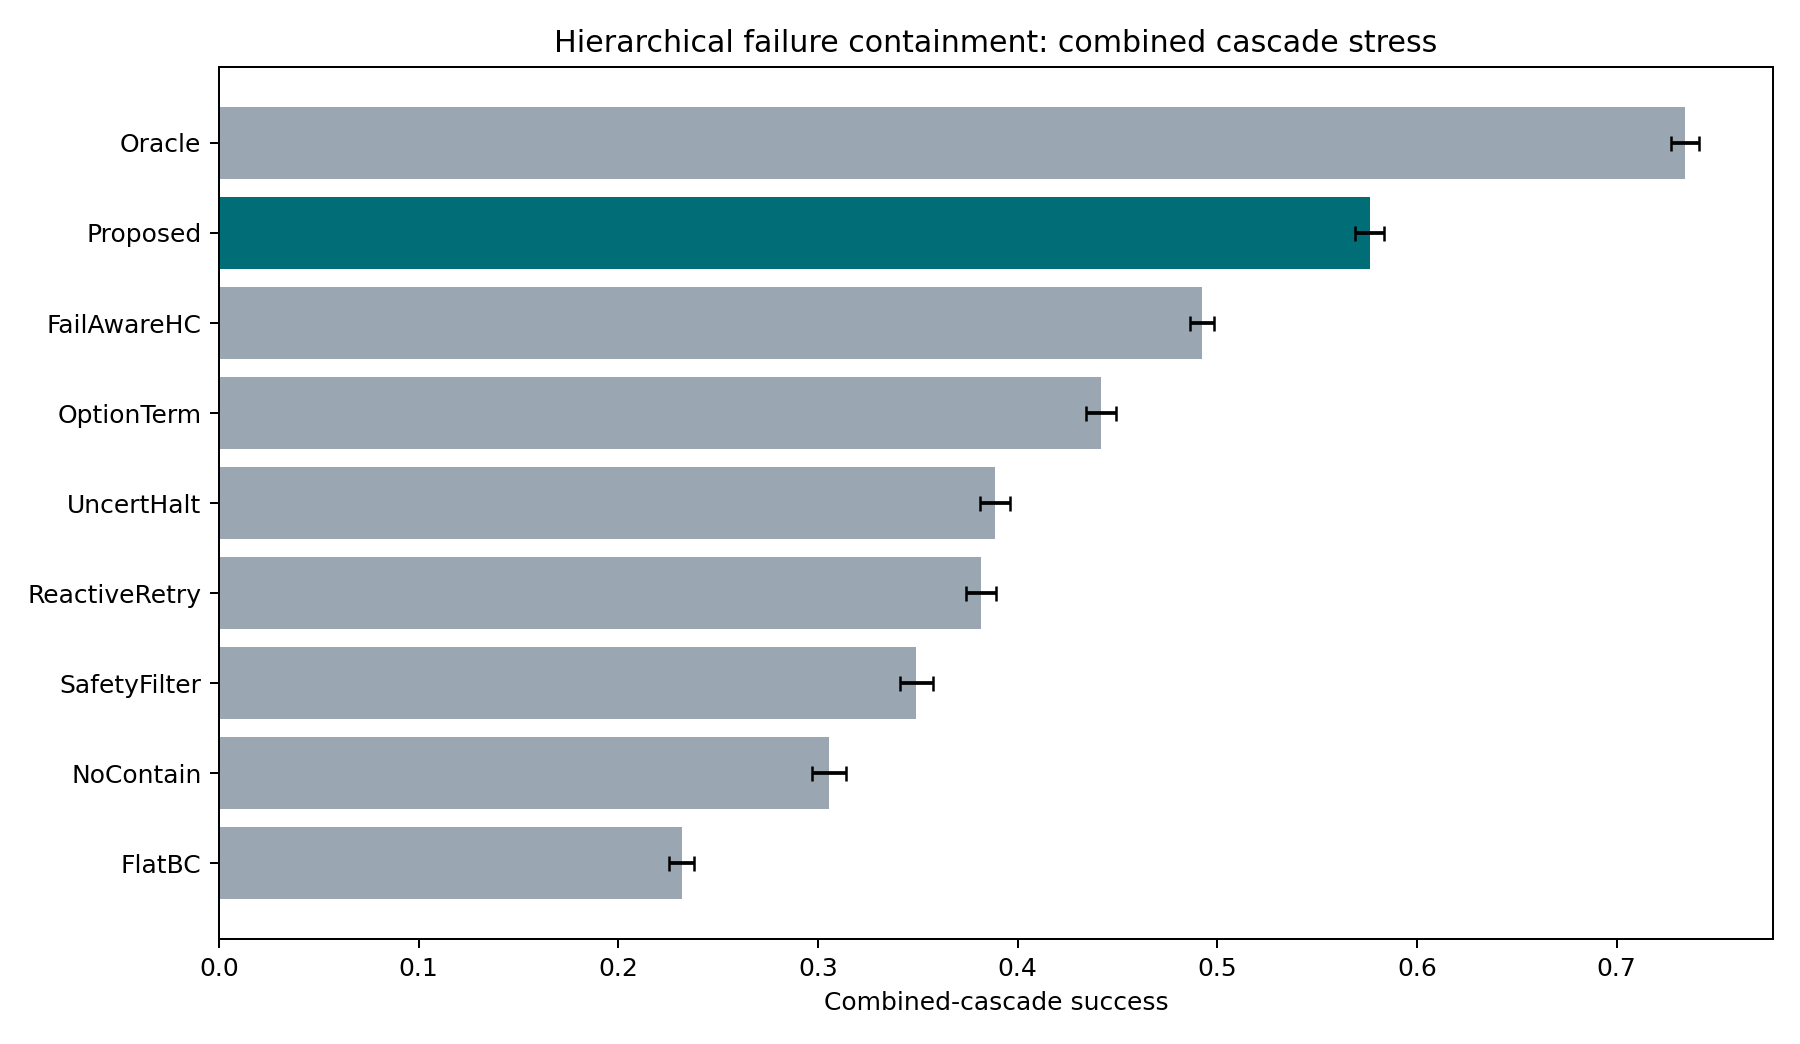
\includegraphics[width=0.95\linewidth]{../figures/hierarchical_containment_combined_success.png}
\caption{Combined-cascade success with 95\% confidence intervals. The proposed containment graph clears the strongest non-oracle baseline but remains below the oracle.}
\end{figure}

\begin{figure}[t]
\centering
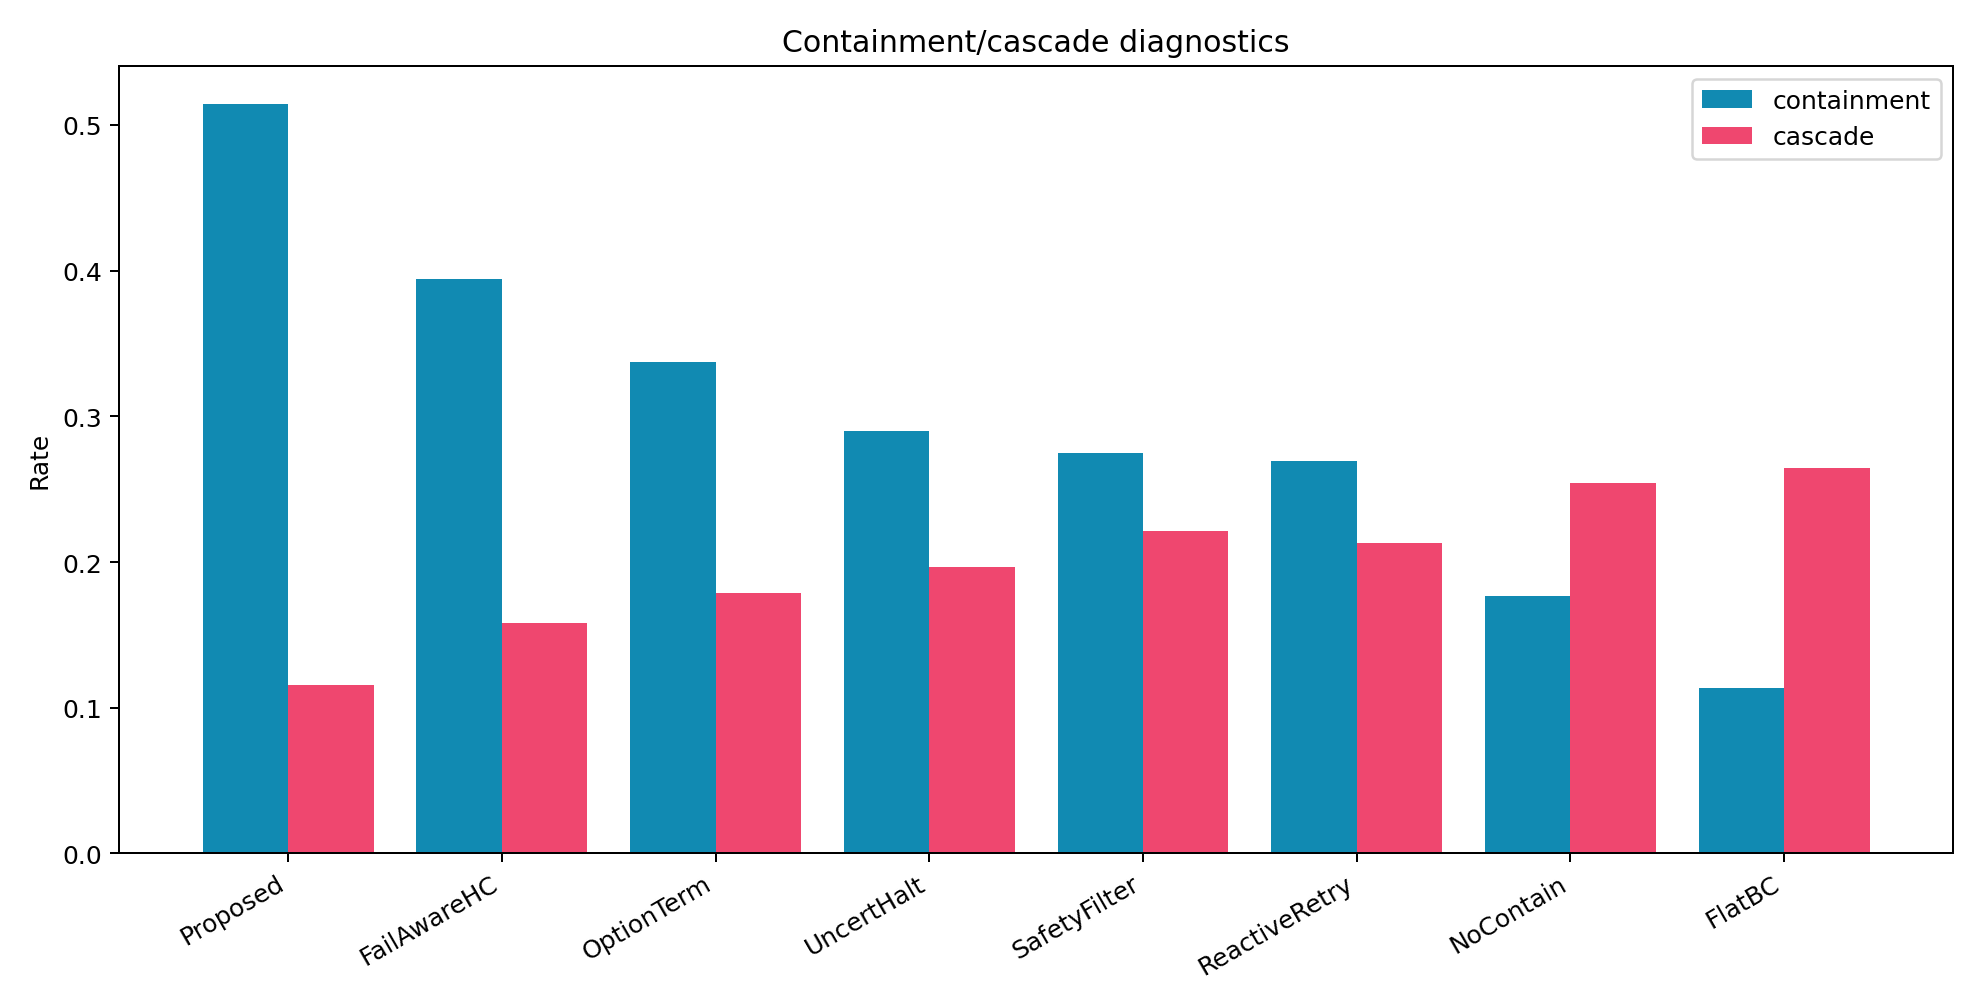
\includegraphics[width=0.95\linewidth]{../figures/hierarchical_containment_diagnostics.png}
\caption{Containment and cascade diagnostics. The proposed method improves the rate of local containment while reducing cross-level cascades.}
\end{figure}

% Auto-generated by src/run_experiment.py
\begin{table}[t]
\centering
\caption{Pairwise combined-cascade success differences against the proposed method.}
\begin{tabular}{lrrr}
\toprule
Baseline & Diff & CI & Wins \\
\midrule
FailAwareHC & 0.084 & 0.009 & 7 \\
FlatBC & 0.345 & 0.011 & 7 \\
NoContain & 0.271 & 0.008 & 7 \\
SafetyFilter & 0.227 & 0.013 & 7 \\
OptionTerm & 0.134 & 0.005 & 7 \\
Oracle & -0.158 & 0.010 & 0 \\
ReactiveRetry & 0.195 & 0.010 & 7 \\
UncertHalt & 0.188 & 0.014 & 7 \\
\bottomrule
\end{tabular}
\end{table}


\section{Ablations and stress tests}
% Auto-generated by src/run_experiment.py
\begin{table}[t]
\centering
\caption{Ablations of the hierarchical failure containment graph.}
\begin{tabular}{lrrrr}
\toprule
Ablation & Succ. & Contain & Cascade & Dmg. \\
\midrule
Full & 0.583 & 0.517 & 0.115 & 0.028 \\
NoHaltCalib & 0.551 & 0.494 & 0.122 & 0.033 \\
NoBudgetMem & 0.509 & 0.459 & 0.142 & 0.044 \\
NoEscalation & 0.502 & 0.433 & 0.160 & 0.051 \\
NoLocalEdges & 0.501 & 0.378 & 0.154 & 0.037 \\
NoCorruptPred & 0.496 & 0.476 & 0.135 & 0.054 \\
FlatRecovery & 0.377 & 0.269 & 0.211 & 0.072 \\
\bottomrule
\end{tabular}
\end{table}


The best removed-component ablation is \texttt{minus\_false\_halt\_calibration}, which still trails the full graph by $0.032$ success. Removing recovery-budget memory, cross-level escalation, local containment edges, or corruption prediction produces larger drops and different failure signatures. This supports the claim that the method is not just an option-termination heuristic or a conservative safety filter.

\begin{figure}[t]
\centering
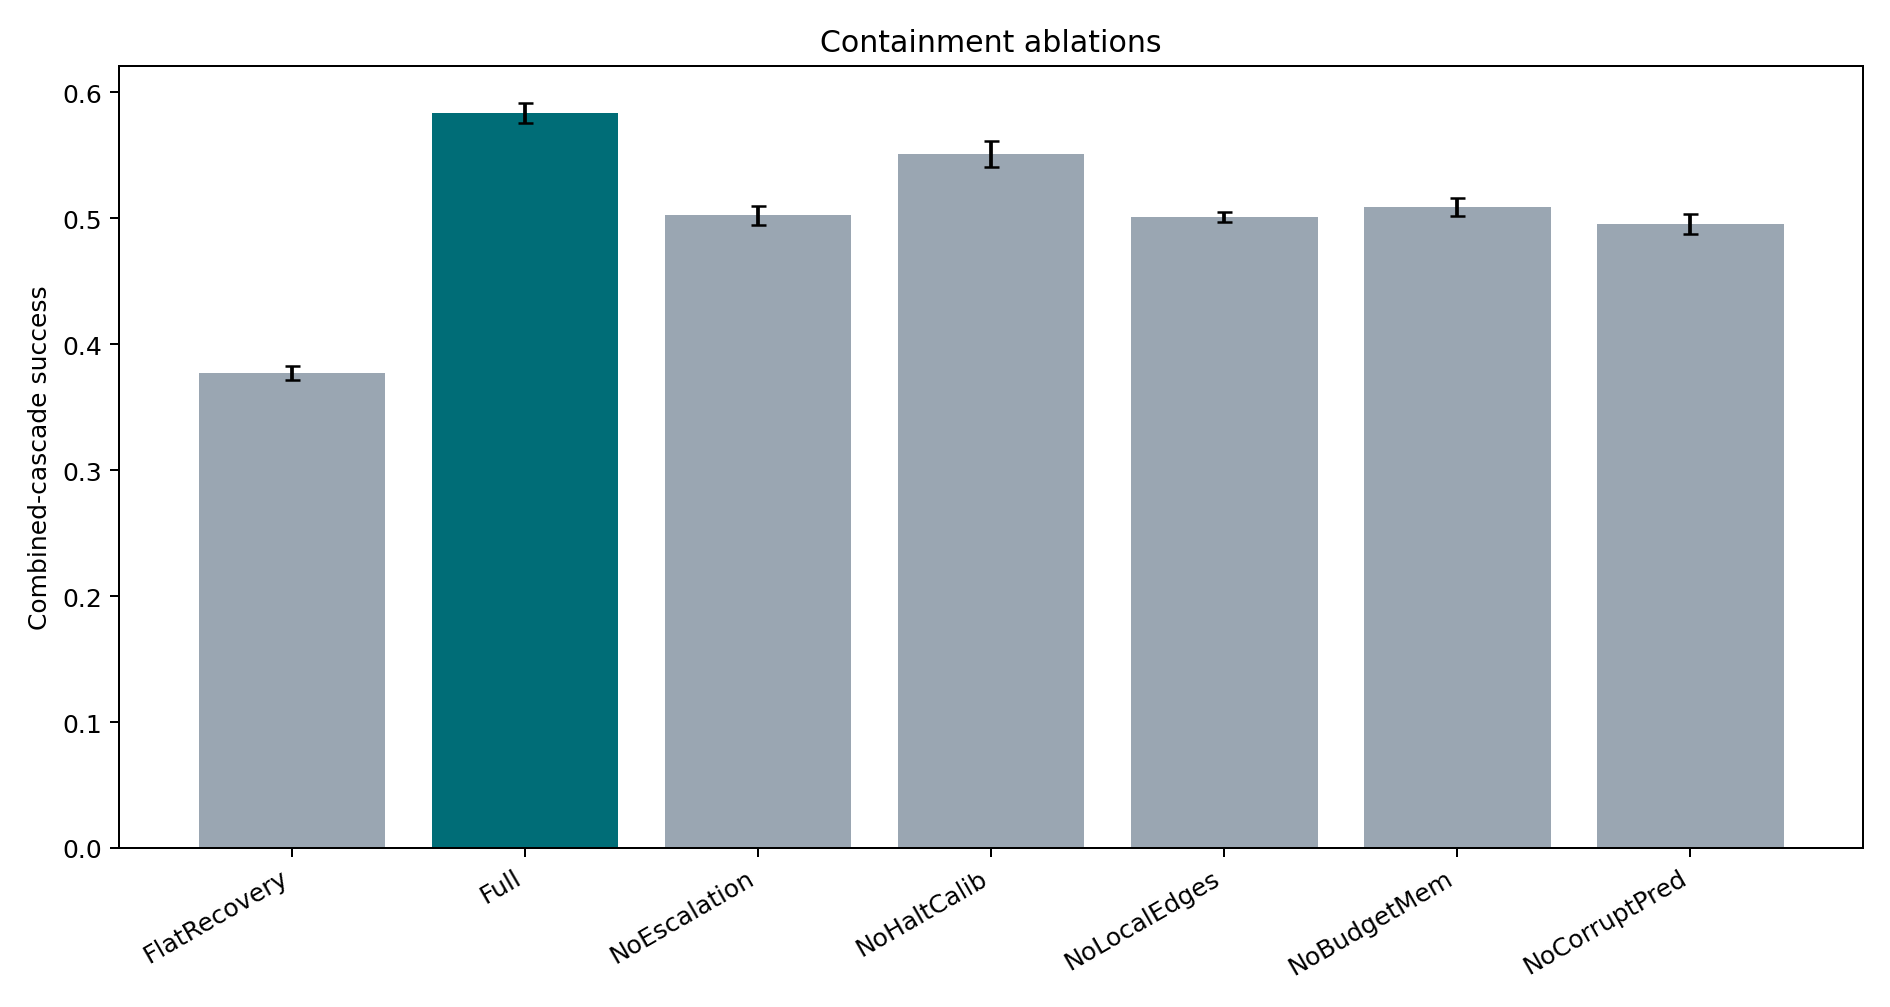
\includegraphics[width=0.95\linewidth]{../figures/hierarchical_containment_ablation.png}
\caption{Ablation success under combined cascade stress. The full graph remains above all removed-component variants.}
\end{figure}

\begin{figure}[t]
\centering
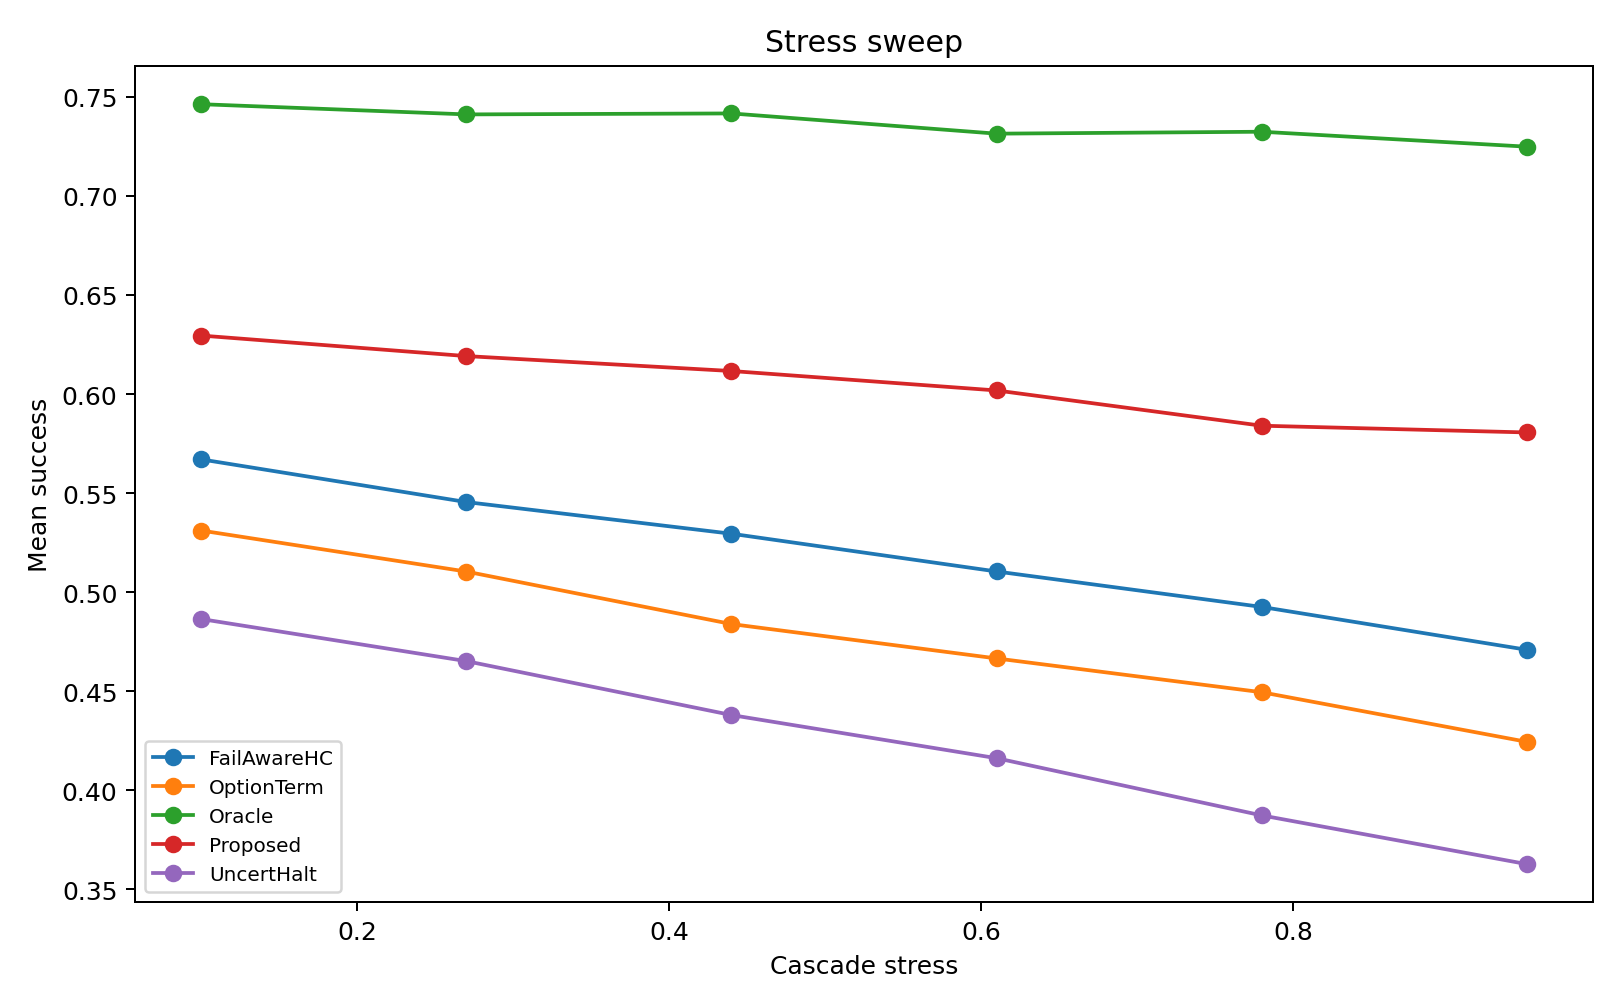
\includegraphics[width=0.95\linewidth]{../figures/hierarchical_containment_stress_sweep.png}
\caption{Stress sweep over cascade intensity. The proposed method remains above non-oracle baselines across the generated stress range, while the oracle remains the ceiling.}
\end{figure}

\begin{figure}[t]
\centering
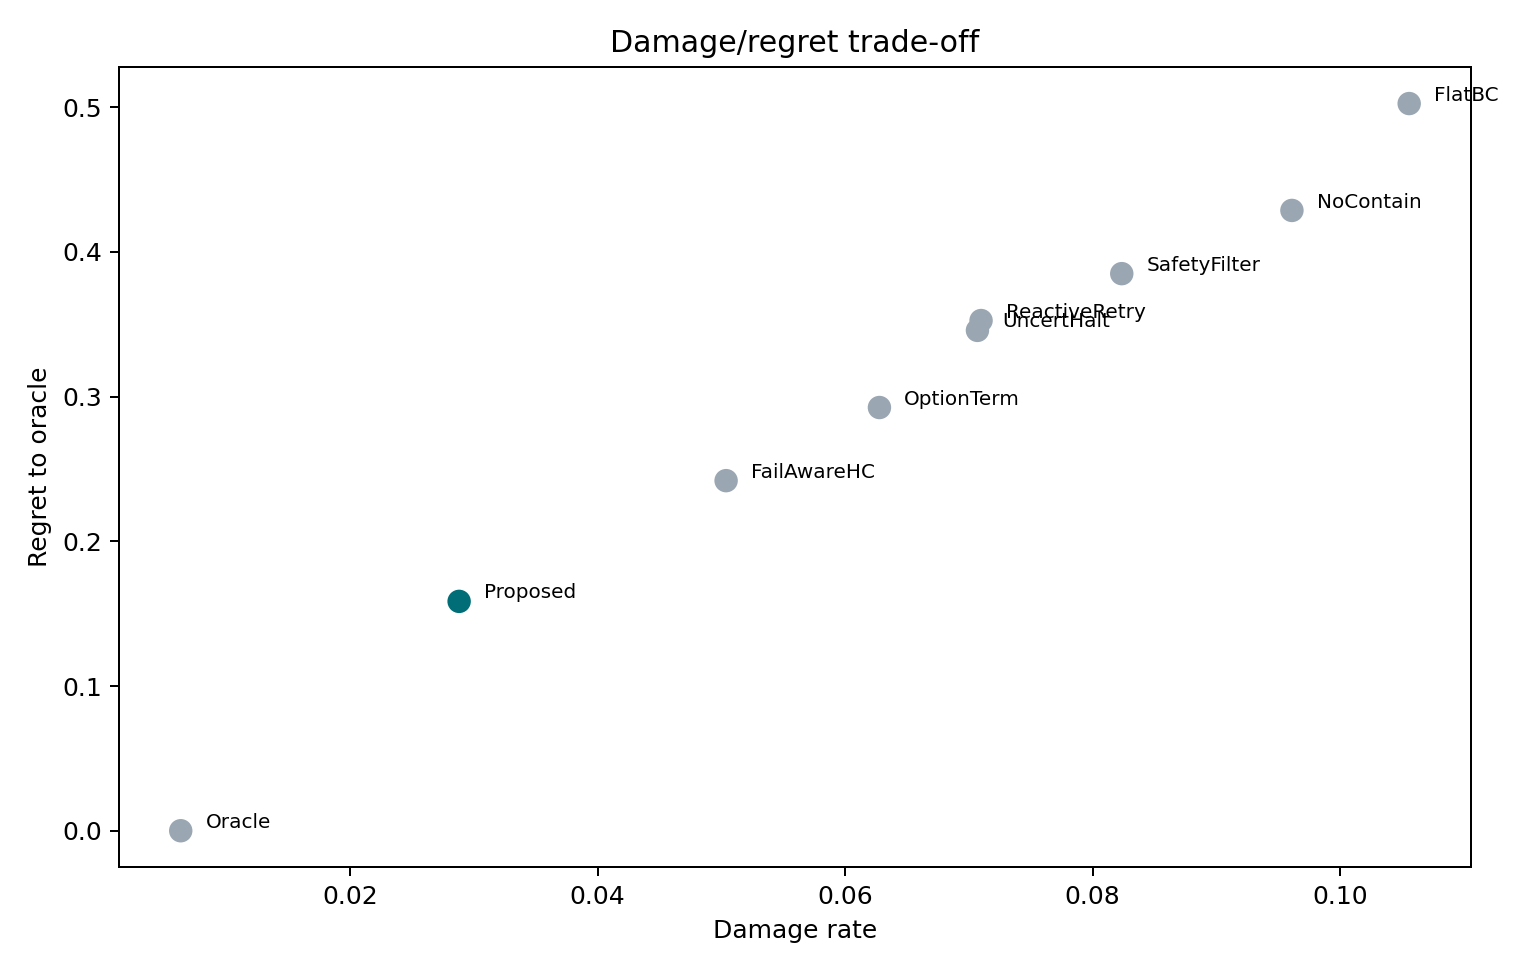
\includegraphics[width=0.95\linewidth]{../figures/hierarchical_containment_damage_regret.png}
\caption{Damage and regret trade-off on combined cascade stress. The proposed method improves task success while lowering damage relative to the strongest non-oracle baseline.}
\end{figure}

\section{Where the method still fails}
The failure-case CSV shows that hierarchical containment helps least when a local retry or option termination can recover before task state is at risk. Those are the intended boundaries. The method's value appears when failures can cross hierarchy levels, recovery budget is limited, or local repair would silently corrupt the high-level task state.

\section{Hostile prior-work boundary}
Options and Option-Critic already provide hierarchical termination machinery \citep{sutton1999options,bacon2017option}. HIRO already learns efficient hierarchical policies \citep{nachum2018hiro}. Recovery RL and RecoveryChaining already introduce learned recovery policies, including manipulation recovery and physical robot transfer \citep{thananjeyan2020recovery,vats2024recoverychaining}. FailSafe and related VLA recovery work already reason about manipulation failures and executable recovery actions \citep{lin2025failsafe}.

The present paper survives only under a narrower interpretation: it is about \emph{containment boundaries}, not hierarchy, termination, recovery, or safety filtering in general. If real robot experiments later show that option termination, failure-aware hierarchy, recovery RL, or simple uncertainty halting match the proposed method on cascade containment without extra damage or false halts, the claim should be killed.

\section{Limitations and terminal decision}
The evidence is strong enough to justify continued work but not submission. The limitations are material:
\begin{itemize}
\item the benchmark is local and synthetic;
\item no real robot or independent high-fidelity simulator has been used;
\item baselines are executable diagnostic models, not external trained robot systems;
\item no learned policy checkpoint, training curve, or deployment video is provided;
\item no external benchmark such as LIBERO, RLBench, Meta-World, BridgeData, or a hardware manipulation suite is reported.
\end{itemize}

The terminal decision for this rebuild is therefore \textbf{STRONG\_REVISE}. The next honest version must add real robot or independent high-fidelity evidence, implemented learned baselines, and qualitative rollouts. Without that evidence, the paper should not be submitted to ICLR main.

\begingroup
\raggedright
\bibliographystyle{iclr2026_conference}
\bibliography{references}
\endgroup

\end{document}
